\newpage
\subsection{Caso d'uso UC3: Registrazione utente }
\label{UC3}
\begin{figure}[ht]
	\centering
	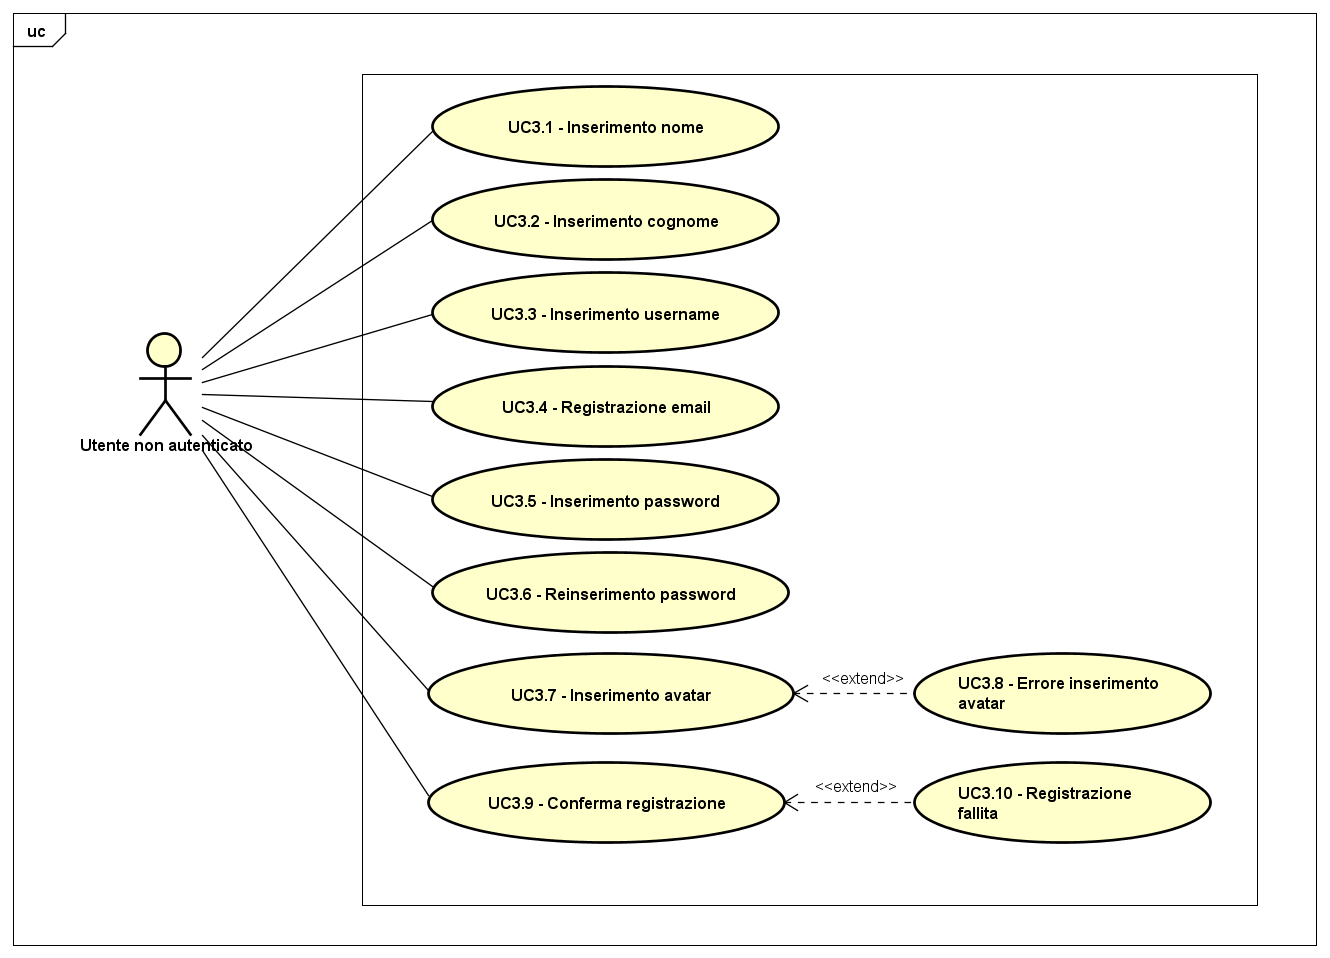
\includegraphics[scale=0.45]{UML/UC3.png}
	\caption{UC3: Registrazione utente}
\end{figure}

\begin{longtable}{ l | p{11cm}}
	\hline
	\rowcolor{Gray}
	 \multicolumn{2}{c}{UC3 - Registrazione utente} \\
	 \hline
	\textbf{Attori} & Utente non autenticato \\
	\textbf{Descrizione} & L'attore inserisce le sue informazioni personali per potersi registrare all'applicazione web, così da poter successivamente effettuare il login ed evolversi in un utente autenticato. \\
	\textbf{Pre-Condizioni} & L'attore ha scelto di registrarsi e l'applicazione web mostra la schermata di registrazione \\
	\textbf{Post-Condizioni} & L'attore si è registrato all'applicazione web \\
	\textbf{Scenario Principale} & \begin{enumerate*}[label=(\arabic*.),itemjoin={\newline}]
		\item L'attore può inserire il proprio nome (UC3.1)
		\item L'attore può inserire il proprio cognome (UC3.2)
		\item L'attore può inserire lo username desiderato (UC3.3)
		\item L'attore può inserire la propria email (UC3.4) 
		\item L'attore può inserire la password desiderata (UC3.5)
		\item L'attore può reinserire la password desiderata per conferma (UC3.6)
		\item L'attore può confermare la registrazione (UC3.7)
	\end{enumerate*}\\
	\textbf{Scenari Alternativi} & 
	\begin{enumerate*}[label=(\arabic*.),itemjoin={\newline}]
		\item L'attore può visualizzare un messaggio d'errore che segnala i campi dati non validi (UC3.8)
	\end{enumerate*}\\
\end{longtable}